\documentclass{article}
\usepackage{preamble}

\title{Unit 8: Curved Spacetime}
\author{Astronomy\footnote{Access for free at \href{\openstax}{\openstax}} \hspace{0.1ex} at Cypress Springs High School}
\date{Updated on \today}

\numberwithin{equation}{section}
\setcounter{section}{8}
\numberwithin{figure}{section}

\usepackage{fancyhdr}
\pagestyle{fancy}
\renewcommand{\headrulewidth}{0pt}
\renewcommand{\headruleskip}{0mm}
\fancyfoot[C]{Access for free at \href{\openstax}{\openstax} \hfill \thepage}
\fancyhead{}

\makenoidxglossaries

\newglossaryentry{black hole}{
    name=black hole,
    description={a region in spacetime where gravity is so strong that nothing---not even light---can escape}
}

\newglossaryentry{event horizon}{
    name=event horizon,
    description={a boundary in spacetime such that events inside the boundary can have no effect on the world outside it---that is, the boundary of the region around a black hole where the curvature of spacetime no longer provides any way out}
}

\newglossaryentry{general theory of relativity}{
    name=general theory of relativity,
    description={Einstein's theory relating gravity and the structure (geometry) of space and time}
}

\newglossaryentry{weight}{
    name=weight,
    description={the force of gravity exerted downwards on your body}
}

\newglossaryentry{free fall}{
    name=free fall,
    description={the experience of falling soley under the gravity of a massive object, like the Earth}
}

\newglossaryentry{force}{
    name=force,
    description={a push or pull on an object with a specific magnitude and direction}
}

\newglossaryentry{gravity}{
    name=gravity,
    description={the force that causes things with mass to attract}
}

\newglossaryentry{gravitational wave}{
    name=gravitational wave,
    description={a disturbance in the curvature of spacetime caused by changes in how matter is distributed; gravitational waves propagate at (or near) the speed of light.}
}

\newglossaryentry{singularity}{
    name=singularity,
    description={the point of zero volume and infinite density to which any object that becomes a black hole must collapse, according to the theory of general relativity}
}

\newglossaryentry{spacetime}{
    name=spacetime,
    description={system of one time and three space coordinates, with respect to which the time and place of an event can be specified}
}

\newglossaryentry{weightlessness}{
    name=weightlessness,
    description={an object's appearance of having no weight, possibly due to being in free fall or experiencing zero gravity; experimentally, if you're weightless and you step on a scale, the scale reads zero pounds}
}

\newglossaryentry{principle of equivalence}{
    name=principle of equivalence,
    description={states that in the absence of evidence of a gravitational field, a freely falling frame is indistinguishable from one in zero gravity}
}

\begin{document}

\maketitle

\subsection{Introducing General Relativity} \label{QpSKf3}

Most stars end their lives as white dwarfs or neutron stars, as we discussed in the last Unit. But when a very massive star collapses at the end of its life, not even the mutual repulsion between densely packed neutrons can support the core against its own weight. If the remaining mass of the star's core is more than about three times that of the Sun, our theories predict that no known force can stop it from collapsing forever! Gravity simply overwhelms all other forces and crushes the core until it occupies an infinitely small volume. A star in which this occurs may become one of the strangest objects ever predicted by theory: a black hole.
\vspace{1em}

To understand what a black hole is like and how it influences its surroundings, we need a theory that can describe the action of gravity under such extreme circumstances. To date, our best theory of gravity is the \gls{general theory of relativity}, which is the theory relating gravity and the structure (geometry) of space and time. It put forward in 1916 by Albert Einstein.
\vspace{1em}

General relativity was one of the major intellectual achievements of the twentieth century. If it were music, we would compare it to the great symphonies of Mozart or Beethoven. Until recently, however, scientists had little need for a better theory of gravity, because Isaac Newton's ideas that led to his law of universal gravitation are perfectly sufficient for most of the objects we deal with in everyday life. But in the past half century, general relativity has become more than just a beautiful idea. It is now essential in understanding pulsars, quasars, and many other astronomical objects and events, including the black holes we will discuss here.
\vspace{1em}

A disclaimer: General relativity involves very advanced mathematics. However, you shouldn't worry, because that math is beyond the scope of this class. Although the detailed calculations of general relativity do involve a good deal of higher mathematics, the basic ideas are not difficult to understand. In fact, they are poetic in the way they give us a new perspective on the world. In addition, general relativity goes beyond Newton's famous ``inverse-square'' law of gravity, by helping explain \textit{how} matter interacts with other matter in space and time. This explanatory power is one of the requirements that any successful scientific theory must meet.

\cyanhrule

\subsection*{\ref{QpSKf3} Exercises}

\begin{exercise} \label{iIb9Ml}
What is the general theory of relativity?
\end{exercise}

\begin{exercise}
    Who first developed the general theory of relativity, and in what year?
\end{exercise}

\begin{exercise}
    Why did scientists, for the longest time, have little need of general relativity to explain gravity?
\end{exercise}

\cyanhrule

\clearpage
\subsection*{The Principle of Equivalence} \label{FSL2KJ}

\Gls{weight} is the force of gravity exerted downwards on your body. The doctor measures your weight when you step on a scale, and you feel the weight of your dog when you pick him up. \Gls{free fall} is the experience of falling under the gravity of a massive object, like the Earth.  \Gls{weightlessness} is an object's state of having zero weight due to experiencing zero gravity, which occurs when the object is very far away from massive bodies. The fundamental insight that led to the formulation of the general theory of relativity starts with a very simple thought relating free fall and weight: if you were able to jump off a high building and fall freely, you would not feel your own weight. In this chapter, we will describe how Einstein built on this idea to reach sweeping conclusions about the very fabric of space and time itself. He called it the ``happiest thought of my life.''
\vspace{1em}

Einstein himself pointed out an everyday example that illustrates this effect. Notice how your weight seems to be \textit{reduced} in a high-speed elevator when it accelerates from a stop to a rapid descent. Similarly, your weight seems to \textit{increase} in an elevator that starts to move quickly upward. This effect is not just a feeling you have: if you stand on a scale in such an elevator, you can measure your weight changing. You can actually perform this experiment in some science museums.
\vspace{1em}

In a \textit{freely falling} elevator, in the absence of air resistance, you would lose your weight altogether. It would appear no different from the state of \gls{weightlessness}. But this is a contradiction. How could you be weightless
% We generally don't like to cut the cables holding elevators to try this experiment, but near-weightlessness can be achieved by taking an airplane to high altitude and then dropping rapidly for a while. This is how NASA trains its astronauts for the experience of free fall in space. The scenes of weightlessness in the 1995 movie \textit{Apollo 13} were filmed in the same way. (\href{https://youtu.be/2V9h42yspbo}{link})
\vspace{1em}

Another way to state Einstein's idea is this: Suppose we have a spaceship that contains a windowless laboratory equipped with all the tools needed to perform scientific experiments. An astronomer finds herself sealed into this windowless laboratory and notices that she is weightless! With her literal window to the external world sealed off from her, she makes a list of possible explanations for why she is weightless. 

\begin{enumerate}
\setlength\itemsep{0.1ex}
    \item She and the laboratory are far away from any source of gravity. Both are either at rest or moving at some steady speed through space. (This is the boring scenario.)
    \item She and the laboratory are falling freely toward a planet like Earth. (This is the terrifying scenario.)
\end{enumerate}

Einstein postulated that \textbf{there is no experiment she can perform inside the sealed laboratory to determine whether she is floating in space or falling freely in a gravitational field}. As far as she is concerned, the two situations are completely equivalent. This idea that free fall is indistinguishable from and equivalent to zero gravity is called the equivalence principle:

\begin{mdframed}[backgroundcolor=black!10]
\textbf{Principle of Equivalence}: 
For a weightless observer in a closed reference frame, it is impossible to determine whether the frame is in free fall or in a region of zero gravity. Therefore, free fall is indistinguishable from and equivalent to zero gravity.

% Since, in an isolated reference frame in which objects appear to be weightless, it is not possible to attain evidence that the frame is a gravitational field, free fall must be indistinguishable from and equivalent to zero gravity.
\end{mdframed}

\cyanhrule

\subsection*{\ref{FSL2KJ} Exercises}

\begin{exercise}
    What is free fall?
\end{exercise}

\begin{exercise}
    What is weight?
\end{exercise}

\begin{exercise}
    What happens to your weight in a freely falling elevator?
\end{exercise}

\begin{exercise}
    What did Einstein postulate about the scientist in a windowless laboratory in space?
\end{exercise}

\begin{exercise} \label{l6wd5D}
    Create your own definition of the principle of equivalence \textit{without} using the word ``indistinguishable.'' Find another word or phrase that means the same ``indistinguishable.''
\end{exercise}

\cyanhrule

\clearpage

\subsection*{Gravity or Acceleration?}

\begin{minipage}{0.53\textwidth}
Einstein's simple idea has big consequences. Let's begin by considering what happens if two foolhardy people jump from opposite banks into a bottomless chasm. Also, pretend there is no air, which means they don't feel the air resistance a skydiver would feel. Then while they freely fall, they both accelerate downward at the same rate and feel no external force acting on them. They can throw a ball back and forth, always aiming it straight at each other, as if there were no gravity. The ball falls at the same rate that they do, so it always remains in a line between them.
\vspace{1em}

But on the surface of Earth, such a game of catch is very different.  Everyone who grows up feeling gravity knows that a ball, once thrown, falls to the ground. Thus, in order to play catch with someone, you must aim the ball upward so that it follows an arc---rising and then falling as it moves forward---until it is caught at the other end.
\vspace{1em}

Now suppose we isolate our falling people and ball inside a large box that is falling with them. No one inside the box is aware of any gravitational force. If they let go of the ball, it doesn't fall to the bottom of the box or anywhere else but merely stays there or moves in a straight line, depending on whether it is given any motion.
\end{minipage}%
\hspace{5mm}
\begin{minipage}{0.37\textwidth}
\centering
    \includegraphics[width=6cm]{Figures/Figure24.4.jpg}
\end{minipage}
\vspace{1em}

Astronauts in the International Space Station (ISS) that is orbiting Earth live in an environment just like that of the people sealed in a freely falling box. The orbiting ISS is actually ``falling'' freely around Earth. While in free fall, the astronauts live in a strange world where there seems to be no gravitational force. One can give a wrench a shove, and it moves at constant speed across the orbiting laboratory. A pencil set in midair remains there as if no force were acting on it.
\vspace{1em}

Appearances are misleading, however. There is a force in this situation. An external observer would see that both the ISS and the astronauts continually fall around Earth, pulled by its gravity. But since all fall together---shuttle, astronauts, wrench, and pencil---inside the ISS all gravitational forces appear to be absent.
\vspace{1em}

Thus, the orbiting ISS provides an excellent example of the principle of equivalence---how \textit{local effects of gravity can be completely compensated by the right acceleration}. To the astronauts, falling around Earth creates the same effects as being far off in space, remote from all gravitational influences.

\cyanhrule

\subsection*{Exercises}

\begin{exercise} \label{MiCFJv}
    When two players are playing catch on the ground on Earth, \textit{how} do they know they are in the presence of a (Earth's) gravitational field? Explain. (\textit{Hint}: Discuss the path taken by the ball, from their perspective.)
\end{exercise}

\begin{exercise} \label{6n6goF}
    Yes or no? When two players are isolated in a large box that is in free fall, do they know whether or not they are in a gravitational field? (\textit{Hint}: Again, discuss the path taken by the ball, from their perspective.)
\end{exercise}

\clearpage
\subsection*{The Paths of Light and Matter}

The greatest consequence of the principle of equivalence is that \textit{experiments conducted in zero gravity must yield the same results as experiments conducted in free fall where gravity is present}.
\vspace{1em}

Einstein postulated that the equivalence principle is a fundamental fact of nature, and that there is no experiment inside any spacecraft by which an astronaut can ever distinguish between being weightless in remote space and being in free fall near a planet like Earth. This would apply to experiments done with beams of light as well. But the minute we use light in our experiments, we are led to some very disturbing conclusions. Such conclusions lead Einstein and us to general relativity and a new view of gravity.
\vspace{1em}

From everyday experience, we know that beams of light travel in straight lines. Imagine that a spaceship is moving through empty space far from any gravity. Send a laser beam from the back of the ship to the front, and it will travel in a nice straight line and land on the front wall exactly opposite the point from which it left the rear wall. If the equivalence principle really applies universally, then this same experiment performed in free fall around Earth should give us the same result.
\vspace{1em}

Now imagine that the astronauts again shine a beam of light along the length of their ship. But, as shown below, this time the orbiting space station falls a bit between the time the light leaves the back wall and the time it hits the front wall. (The amount of the fall is exaggerated in the figure to illustrate the effect.) Therefore, if the beam of light follows a straight line but the ship's path curves downward, then the light should strike the front wall at a point higher than the point from which it left.

% \begin{figure}[h!]
%     \centering
%     \includegraphics[width=10cm]{Figures/Figure24.6.jpg}
% \end{figure}

\begin{center}
\textbf{ZERO GRAVITY}
\vspace{1ex}

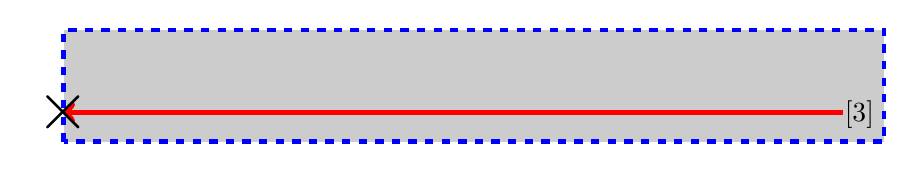
\begin{tikzpicture}
\begin{axis}[
    width=12cm,
    height=3cm,
    xmin=0,xmax=10,ymin=0,ymax=5,
    ticks=none,
    axis lines=left,
    clip=false,
    axis line style={draw=none},
]
    \draw[ultra thick,blue,dashed,fill=black!20] (0,0) rectangle (10,5);
    \node at (9.7,1.2) {\Strichmaxerl[3]};
    \draw[ultra thick,red,->] (9.5,1.3) -- ++(axis direction cs: -9.5,0); 
    \node at (0,1.3) {\Huge $\times$};
\end{axis}
\end{tikzpicture}
\end{center}
\vspace{1em}

\hrule

\vspace{1em}

\begin{center}
\textbf{FREE FALL}
\vspace{1ex}

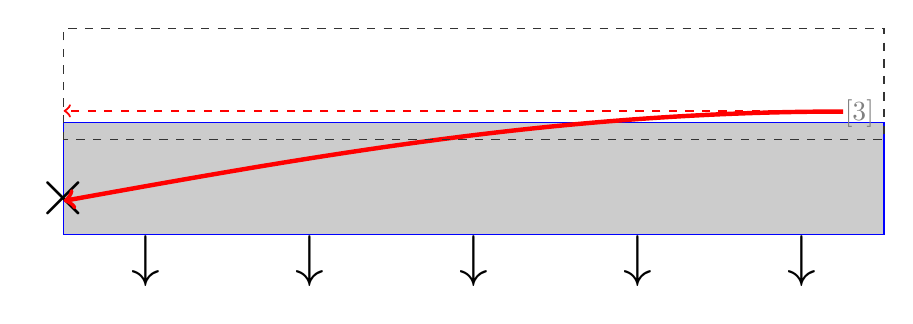
\begin{tikzpicture}
\begin{axis}[
    width=12cm,
    height=3cm,
    xmin=0,xmax=10,ymin=0,ymax=5,
    ticks=none,
    axis lines=left,
    clip=false,
    axis line style={draw=none},
]
    \begin{scope}[yshift=-1.2cm]
        \draw[blue,fill=black!20] (0,0) rectangle (10,5);
        \node at (0,1.6) {\Huge $\times$};
        \draw[red,<-,ultra thick] (0,1.5) sin +(9.5,4);
        \node at (1,-1.2) {\huge $\downarrow$};
        \node at (3,-1.2) {\huge $\downarrow$};
        \node at (5,-1.2) {\huge $\downarrow$};
        \node at (7,-1.2) {\huge $\downarrow$};
        \node at (9,-1.2) {\huge $\downarrow$};
    \end{scope}
    \node at (9.7,1.2) {\color{gray} \Strichmaxerl[3]}; 
    \draw[dashed,black!80] (0,0) rectangle (10,5);
    \draw[thick,red,dashed,->] (9.5,1.3) -- ++(axis direction cs: -9.5,0); 
\end{axis}
\end{tikzpicture}
\end{center}


However, this would violate the principle of equivalence because the two experiments would give different results. This means only one of the following assumptions is correct, and the other must be abandoned:

\begin{enumerate}
\setlength\itemsep{-1ex}
    \item Either the principle of equivalence is correct.
    \item Or light always travels in straight lines.
\end{enumerate}

During Einstein's time, the principle of equivalence seemed like a ridiculous idea. Yet Einstein kept this first assumption and instead worked out what happens if light sometimes does \textit{not} follow a straight path.
\vspace{1em}

Let's suppose the principle of equivalence is right. Then the light beam must arrive directly opposite the point from which it started in the ship. The light, like the ball thrown back and forth, must fall with the ship that is in orbit around Earth. This fact would make the light beam's path curve downward, like the path of the ball, so that beam would hit the front wall exactly opposite the spot from which it came.
\vspace{1em}

Thinking this over, you might well conclude that it doesn't seem like such a big problem: why can't light fall the way basketballs do? Because light is profoundly different from basketballs. Basketballs have mass, while light does not.
\vspace{1em}

Here is where Einstein's intuition and genius allowed him to make a profound leap. He gave physical meaning to the strange result of our thought experiment. Einstein suggested that the light curves down to meet the front of the shuttle because \textit{Earth's gravity actually bends the fabric of space and time}. This radical idea keeps the behavior of light the same in both empty space and free fall, but it changes some of our most basic and cherished ideas about space and time. The reason we take Einstein's suggestion seriously is that, as we will see, experiments now clearly show his intuitive leap was correct.

\cyanhrule

\subsection*{Exercises}

\begin{exercise} \label{vEYTBu}
    What is one great consequence of the principle of equivalence regarding experiments performed in zero gravity?
\end{exercise}

\begin{exercise}
    From your everyday experience, what is the shape of the path of a light ray? (Think of using a laser to shine a point on the wall.)
\end{exercise}

\begin{exercise}
    Pretend you are in a spaceship far away in a zero gravity environment. If you shine a red laser horizontally at a height of 1.5 meters towards the opposite wall, at what height will it hit the opposite wall?
\end{exercise}

\begin{exercise}
    Now suppose your spaceship is in free fall near the gravity of a massive object and you shine the same laser at the same height. The laser hits the same spot that it hit in the zero gravity experiment. Is the path of the light a straight line?
\end{exercise}

\begin{exercise}\label{XFnLZe}
    What does Earth's gravity do to the ``fabric'' of space and time?
\end{exercise}

\clearpage
\subsection{Tests of General Relativity}

What Einstein proposed was nothing less than a major revolution in our understanding of space and time. It was a new theory of gravity, in which mass determines the curvature of spacetime and that curvature, in turn, controls how objects move. Like all new ideas in science, no matter who advances them, Einstein's theory had to be tested by comparing its predictions against the experimental evidence. This was quite a challenge because the effects of the new theory were apparent only when the mass was quite large. (For smaller masses, it required measuring techniques that would not become available until decades later.)
\vspace{1em}

When the distorting mass is small, the predictions of general relativity must agree with those resulting from Newton's law of universal gravitation, which, after all, has served us admirably in our technology and in guiding space probes to the other planets. In familiar territory, therefore, the differences between the predictions of the two models are subtle and difficult to detect. Nevertheless, Einstein was able to demonstrate one proof of his theory that could be found in existing data and to suggest another one that would be tested just a few years later.

\subsubsection*{The Motion of Mercury}

Of the planets in our solar system, Mercury orbits closest to the Sun and is thus most affected by the distortion of spacetime produced by the Sun's mass. Einstein wondered if the distortion might produce a noticeable difference in the motion of Mercury that was not predicted by Newton's law. It turned out that the difference was subtle, but it was definitely there. Most importantly, it had already been measured.
\vspace{1em}

Mercury has a highly elliptical orbit, so that it is only about two-thirds as far from the Sun at perihelion as it is at aphelion. (These terms were defined in the chapter on Orbits and Gravity.) The gravitational effects (perturbations) of the other planets on Mercury produce a calculable advance of Mercury's perihelion. What this means is that each successive perihelion occurs in a slightly different direction as seen from the Sun.
\vspace{1em}

According to Newtonian gravitation, the gravitational forces exerted by the planets will cause Mercury's perihelion to advance by about 531 seconds of arc (arcsec) per century. In the nineteenth century, however, it was observed that the actual advance is 574 arcsec per century. The discrepancy was first pointed out in 1859 by Urbain Le Verrier, the co-discoverer of Neptune. Just as discrepancies in the motion of Uranus allowed astronomers to discover the presence of Neptune, so it was thought that the discrepancy in the motion of Mercury could mean the presence of an undiscovered inner planet. Astronomers searched for this planet near the Sun, even giving it a name: Vulcan, after the Roman god of fire. (The name would later be used for the home planet of a famous character on a popular television show about future space travel.)
\vspace{1em}

But no planet has ever been found nearer to the Sun than Mercury, and the discrepancy was still bothering astronomers when Einstein was doing his calculations. General relativity, however, predicts that due to the curvature of spacetime around the Sun, the perihelion of Mercury should advance slightly more than is predicted by Newtonian gravity. The result is to make the major axis of Mercury's orbit rotate slowly in space because of the Sun's gravity alone. The prediction of general relativity is that the direction of perihelion should change by an additional 43 arcsec per century. This is remarkably close to the observed discrepancy, and it gave Einstein a lot of confidence as he advanced his theory. The relativistic advance of perihelion was later also observed in the orbits of several asteroids that come close to the Sun.

\subsection*{Exercises}

\begin{exercise}
    Of all the planets, why is Mercury the most affected by the distortion of spacetime produced by the Sun's mass?
\end{exercise}

\begin{exercise}
    According to Einstein, what happens to Mercury as it orbits the curved spacetime near the Sun?
\end{exercise}

\begin{exercise}
    What does it mean that Mercury's orbit is ``highly elliptical''? Draw a rough sketch of its orbit.
\end{exercise}

\begin{exercise}
    What does \textit{perihelion} mean? Draw a sketch of Mercury's perihelion.
\end{exercise}

\begin{exercise}
    According to Newtonian gravitation, the gravitational forces exerted by the planets will cause Mercury's perihelion to advance by about 531 seconds of arc (arcsec) per century. Arcseconds are units of angles, like the ``degrees'' you learned about in geometry, but they're much smaller. 1 arcsecond equals $\frac{1}{3600}$ degrees. Divide the number above by 3600 to convert that measurement to degrees.
\end{exercise}

\begin{exercise}
    As observed in 1859 by Urbain Le Verrier, what was the actual advance per century of Mercury's perihelion? State your answer in arcseconds and in degrees. (Divide arcseconds by 3600 to get degrees).
\end{exercise}

\begin{exercise}
    As early as 1859, way before Einstein, astronomers observed that Mercury's orbit varied slightly from predictions made by Newton's law of universal gravitation. They (falsely) believed this variation was caused by an undiscovered inner planet. What did they name this planet?
\end{exercise}

\clearpage
\subsection*{Deflection of Starlight}

\begin{center}
    \includegraphics[width=0.8\textwidth]{Figures/Figure24.10.jpg}
\end{center}

\subsection*{Exercises}

\href{https://youtu.be/HLxvq_M4218}{Click here} to watch a video. 

% \begin{exercise}
%     Isaac Newton published his laws of physics in his book \textit{Principia} in the year \rule{2cm}{0.15mm} .
% \end{exercise}

\begin{exercise}
    In opposition to Newton, Einstein saw gravity as something completely \rule{2cm}{0.15mm}. 
\end{exercise}

\begin{exercise}
    Einstein said that massive objects, like the Sun, \rule{2cm}{0.15mm} the space around them.
\end{exercise}

\begin{exercise}
    What was one of the conflicts that prevented Einstein from testing the deflection of starlight by the Sun?
\end{exercise}

\begin{exercise}
    Which British astronomer set out to test Einstein's prediction?
\end{exercise}

\begin{exercise}
    The eclipse in May of the year \rule{2cm}{0.15mm} was the ideal opportunity to test the deflection of starlight.
\end{exercise}

\begin{exercise}
    What two locations were chosen to observe the eclipse?
\end{exercise}

\begin{exercise}
    When Eddington compared the photograph of the eclipse to the photograph of the night sky, he notice that the stars are \rule{2cm}{0.15mm} during the eclipse.
\end{exercise}

\begin{exercise}
    In what year was the first photograph of a black hole taken?
\end{exercise}

\clearpage

\subsection{Black Holes}

A \gls{black hole} is a a region in spacetime where gravity is so strong that nothing---not even light---can escape. The \gls{event horizon} is a boundary in spacetime such that events inside the boundary can have no effect on the world outside it---that is, the boundary of the region around a black hole where the curvature of spacetime no longer provides any way out. A \gls{singularity} is the point of zero volume and infinite density to which any object that becomes a black hole must collapse, according to the theory of general relativity.

\clearpage

\subsection{Relevant Application: Short Story About a Journey to a Black Hole} \label{hxYdNl}

\subsubsection*{Objectives}

\begin{itemize}
\setlength\itemsep{-1ex}
    \item To review this unit on curved spacetime by summarizing key points and terms in a short story
    \item To create a compelling story about the journey to a black hole
\end{itemize}

\subsubsection*{Procedure}

\begin{enumerate}
\setlength\itemsep{-1ex}
    \item Join a group of no more than 3 people. Designate one group member as the \textbf{artist}, who will draw or design illustrations for the short story; one member as the \textbf{writer}, who creates the main components of the story line; and one member as the \textbf{producer}, who compiles the illustrations and text in a nicely formatted Google Slides show.
    \item Your story must contain at least one mention of each of the following vocabulary words from this unit: \gls{black hole}, \gls{event horizon}, \gls{free fall}, \gls{general theory of relativity}, \gls{principle of equivalence}, \gls{singularity}, \gls{weight}, and \gls{weightlessness}.
    \item Your story must contain a beginning, middle, and end. Make it as well-written, exciting, and memorable as you can. Although the writer does the bulk of story creation, all group members should have their say in what goes in the story. Give your character(s) a name(s). Be descriptive in your language.
\end{enumerate}

\subsubsection*{Recommendation}

\begin{itemize}
\setlength\itemsep{-1ex}
    \item In class, we told you that spending 2 weeks near the distorted spacetime of a certain black hole is equivalent to 2000 weeks on Earth, and that in a sense time travel is possible because your friends back on Earth would have aged 20 more years by the time you get back. You should consider adding this element of time distortion to your story.
\end{itemize}

\subsubsection*{Submission}

\begin{enumerate}
\setlength\itemsep{-1ex}
    \item All text and illustrations must be added to a \href{https://docs.google.com/presentation/}{Google Slides} presentation. Each slide of the show is like a different page of a book.
    \item When your story is near finished, create a cover slide containing the story's title, an illustration, and the names of all members of your group.
    \item When the story is finalized, it is the producer's responsibility to share the link with the teacher via Schoology so that all group members get credit.
\end{enumerate}







\clearpage
\printnoidxglossaries

\clearpage
\subsection*{Daily Lesson Plans}

\begin{tabular}{|m{0.25\textwidth}|m{0.7\textwidth}|}
    \hline  
    \cellcolor{black!20}\textbf{Date} &
    \cellcolor{black!20}\textbf{Wednesday, January 25, 2023} \\
    \hline
    Learning Intention (TPO) & We introduce the \gls{general theory of relativity}. \\
    \hline
    Hook/Warm Up/Opening & In previous unit, we talked about two types of deaths of stars. They become a white dwarf (which the Sun will) or a neutron star. In this unit we will discuss a third possible outcome: stars leaving behind a black hole. First we need to introduce curved spacetime and general relativity.\\
    \hline
    Lesson/Learning Activities & Introduce \gls{general theory of relativity}, \gls{weight}, \gls{free fall}, and \gls{weightlessness}.\\
    \hline
    Graded Activities & Exercises \#\ref{iIb9Ml}--\ref{l6wd5D}.\\
    \hline
    Closure & Stamp students' completed work, and discuss lingering questions.\\  
    \hline
\end{tabular}  

\begin{tabular}{|m{0.25\textwidth}|m{0.7\textwidth}|}
    \hline  
    \cellcolor{black!20}\textbf{Date} &
    \cellcolor{black!20}\textbf{Thursday, January 26, 2023} \\
    \hline
    Learning Intention (TPO) &  Introduce the \gls{principle of equivalence}\\
    \hline
    Hook/Warm Up/Opening & Watch \href{https://youtu.be/WMK36dpHIkg}{this video} to see motion in the weightless environment of the International Space Station (ISS). \\
    \hline
    Lesson/Learning Activities & Discuss the throught experiment of the weightless astronomer in a windowless laboratory in outer space. Her two conclusions are she is either in free fall near a massive body or she's in a zero gravity region of space. Either way, she can't tell the difference. Define the \gls{principle of equivalence}. Watch \href{https://youtu.be/DjpueFi5Jms}{this video}, also in the ISS, paying careful attention to the straight-line motion of sandwich at the end of the video. Pick 2 student volunteers to help you re-create the straight-line motion of a ball thrown to the other person in a weightless environment.\\
    \hline
    Graded Activities &  Exercises \#\ref{MiCFJv} and \ref{6n6goF}.\\
    \hline
    Closure & Stamp students' completed work, and discuss lingering questions.\\  
    \hline
\end{tabular}

\begin{tabular}{|m{0.25\textwidth}|m{0.7\textwidth}|}
    \hline  
    \cellcolor{black!20}\textbf{Date} &
    \cellcolor{black!20}\textbf{Monday, January 30, 2023} \\
    \hline
    Learning Intention (TPO) &  We will learn the paths of light and matter in curved space time.\\
    \hline
    Hook/Warm Up/Opening & If you could summarize what we've learned so far about General Relativity to a 6th grader, what would you tell them?\\
    \hline
    Lesson/Learning Activities & Lecture. Emphasize that an application of the principle of equivalence is that experiments in zero gravity must produce the same results in free fall. The laser light must bend with spacetime to land in the same spot. Read \textit{General Relativity for Babies} by Chris Ferrie. Watch \href{https://youtu.be/MTY1Kje0yLg}{this video} about visualizing the fabric of spacetime.\\
    \hline
    Graded Activities & Exercises \#\ref{vEYTBu}--\ref{XFnLZe}. \\
    \hline
    Closure & Students submit sticky note with questions about General Relativity.\\  
    \hline
\end{tabular}  

\begin{tabular}{|m{0.25\textwidth}|m{0.7\textwidth}|}
    \hline  
    \cellcolor{black!20}\textbf{Date} &
    \cellcolor{black!20}\textbf{Thursday, Feburary 2, 2023} \\
    \hline
    Learning Intention (TPO) & We will recognize the significance of the 1919 solar eclipse to Einstein's theory of general relativity. \\
    \hline
    Hook/Warm Up/Opening & Open Stellarium. Set location to Cypress, Texas. (1) Find the times that the planets Saturn, Venus, and Jupiter will set below the horizon tonight. (2) Find the times they will rise tomorrow morning.\\
    \hline
    Lesson/Learning Activities & Watch \href{https://youtu.be/HLxvq_M4218}{this video} and discuss 8 questions. \\
    \hline
    Graded Activities & 8 questions. \\
    \hline
    Closure & Discussion of answers.\\  
    \hline
\end{tabular}  

\begin{tabular}{|m{0.25\textwidth}|m{0.7\textwidth}|}
    \hline  
    \cellcolor{black!20}\textbf{Date} &
    \cellcolor{black!20}\textbf{Monday, February 6, 2023} \\
    \hline
    Learning Intention (TPO) &  We will describe black holes and share ideas through an online black hole simulator.\\
    \hline
    Hook/Warm Up/Opening & Notebook entry. \texttt[red]{Do you think it's possible to time travel? Why or why not?} Tell Ss that according to Einstein's general relativity theory, it is physically possible to time travel---but only forward in time. Future time travel is not against the laws of physics. For e.g., you travel for 10 years to a black hole, spend 2 weeks near distorted spacetime, and travel 10 years back. In total, you aged 20 years but everyone on Earth aged 40 years! All your friends will be in much older than you.\\
    \hline
    Lesson/Learning Activities & \textit{Doc camera}. Define \gls{black hole}, \gls{event horizon}, and \gls{singularity}. Define density as the amount of stuff per unit of volume. The density of bread is about \SI{0.25}{g/cm^3}. \href{https://youtu.be/AeJ9q45PfD0}{Aerogels} have densities of about \SI{0.003}{g/cm^3}. Gold's density is \SI{19}{g/cm^3}. Consider that the singularity has infinite density in zero volume. \\
    \hline
    Graded Activities & \\
    \hline
    Closure & \\  
    \hline
\end{tabular}

\begin{tabular}{|m{0.25\textwidth}|m{0.7\textwidth}|}
    \hline  
    \cellcolor{black!20}\textbf{Date} &
    \cellcolor{black!20}\textbf{Tuesday, February, 7 2023} \\
    \hline
    Learning Intention (TPO) & We will summarize curved spacetime and general relativity and share ideas through a creation of an original science fiction story about the journey to a black hole. \\
    \hline
    Hook/Warm Up/Opening & Arrange Ss in self-assigned groups of 3 or less. \\
    \hline
    Lesson/Learning Activities & Explain the assignment's instructions, which are summarized in Section \ref{hxYdNl}. \\
    \hline
    Graded Activities & This assignment is due on Thursday and will be a relevant applications grade.\\
    \hline
    Closure & After a few minutes of group deliberations, walk around and ask the students what their stories will be about. Ensure they have assigned a writer, producer, and artist.\\  
    \hline
\end{tabular}





\end{document}

%%%% Template
\begin{tabular}{|m{0.25\textwidth}|m{0.7\textwidth}|}
    \hline  
    \cellcolor{black!20}\textbf{Date} &
    \cellcolor{black!20}\textbf{***day, Jan, DD 2023} \\
    \hline
    Learning Intention (TPO) & We will [] and share ideas through a/an []. \\
    \hline
    Hook/Warm Up/Opening & \\
    \hline
    Lesson/Learning Activities & \\
    \hline
    Graded Activities & \\
    \hline
    Closure & \\  
    \hline
\end{tabular}  